\documentclass[11pt, titlepage]{article}
\usepackage[a4paper, nomarginpar, total={170mm, 257mm}, left=40mm, right=25mm, top=20mm, bottom=20mm]{geometry}

\usepackage[utf8]{inputenc}
\usepackage[L7x]{fontenc}
\usepackage[lithuanian]{babel}

\usepackage{tgtermes}

\usepackage{graphicx}
\graphicspath{ {./images/} }

\title{INFLIACIJOS IR NEDARBO SĄSAJA LIETUVOJE}
\author{Judilė Bernackaitė}
\date{2019 06 17}

\begin{document}

\maketitle
\newpage
\tableofcontents
\newpage

\section{Įvadas}

Turbūt vieni iš svarbiausių šalies ekonominių rodiklių yra BVP, infliacija, nedarbo lygis bei darbo užmokestis. Tačiau šiuo atveju nagrinėsime tik du rodiklius: infliaciją ir nedarbą.

Kaip apibrėžia V. Skominas knygoje „Makroekonomika“ - infliacija, tai nuolatinis kainų lygio kilimas arba perkamumo pajėgumo mažėjimas. Infliacijos atsiradimas siejamas dar su senovės Romos laikais, kai buvo nuvertinamos auksinės monetos nupjaunant jų dalį \cite{linapaliu2015}. Apie infliacijos naudą ar žalą nėra vienareikšmės nuomonės. Nekontroliuojama infliacija gali nevaldomai didėti ir pasiekti šuoliuojančios infliacijos lygį, t.y. kai infliacija per metus apytiksliai padidėja 11-100 proc. Smarkiai išaugęs infliacijos lygis pakeičia įprastą ekonomikos eigą. Žmonės matydami spartų pinigų nuvertėjimą stengiasi juos investuoti į nekilnojamą turtą, papuošalus, auksą. Didelis infliacijos lygis gali reikšti ekonomikos smukimą. Tačiau būtų netikslu teigti, kad tik didelis infliacijos lygis yra blogai. Sąlyginai mažas arba neigiamas infliacijos lygis – defliacija yra taip pat nėra gerai. Defliacijos metu žmonės gali įpirkti daugiau prekių nei su ta pačia pinigų suma esant normaliai infliacijai. Žmonėms, kurie turi daug santaupų, defliacija gali pasirodyti išties naudinga, tačiau valstybei tai ne ne itin naudinga. Remiantis Europos centrinio banko (ECB) nurodymais šalyse infliacija turėtų būti mažesnė, bet artima 2 proc. \cite{europoscentrinisbankas2017}. Pasak ECB toks infliacijos lygis padėtų išlaikyti sąlyginai stabilias kainas, būtų kaip rezervas, jog infliacija netaptų neigiama taip pat būtų palikta galimybė konkuruoti šalims. Mažas infliacijos lygis taip pat naudingas skolininkams, kurie gražina tą pačia pinigų sumą, tačiau tuo metu ji mažiau vertinga. Taip pat infliacija gali paskatinti produkcijos padidėjimą.

Žmonių pragyvenimui kiekvieną dieną reikalingi pinigai, o pagrindinis jų šaltinis yra darbas. Tikėtina, kad kuo daugiau yra dirbančių žmonių, tuo šalies gyventojų pragyvenimo lygis yra aukštesnis. Tai iš dalies sąlygoja ir aukštesnį ekonomikos lygį šalyje. Todėl nedarbo lygis yra svarbus šalies ekonomikos rodiklis. Nedarbo lygis parodo kokia procentinė dalis šalies žmonių galinčių ir norinčių dirbti neranda darbo. Nors augant ekonomikai, nedarbo lygis mažėjo, tačiau Lietuvoje nedarbo lygis vis dar yra pakankamai aukštas. Tikėtina, kad aukštą nedarbo lygį Lietuvoje išlaiko tai, jog šalyje nemažai žemos kvalifikacijos darbuotojų, kurie turi mažai galimybių įsidarbinti. Kaip rašoma dokumente „KOMISIJOS TARNYBŲ DARBINIS DOKUMENTAS. Šalies ataskaita. Lietuva 2019“ siekis mažinti nedarbą turi trūkumų. Didelė dalis dirbančiųjų sudaro išsilavinę žmonės, tačiau šalyje yra daug žemos kvalifikacijos žmonių. Tokie žmonės nedirba ir nesimoko, taip pat jų dalyvavimas įvairiose programose nėra aktyvus. Nors šalies ataskaitoje ir skelbiama, jog nedarbo lygis nukrito iki 6.3 proc., tačiau pridedama, kad nereiktų pamiršti, jog šalyje taip pat mažėja ir darbingo amžiaus žmonių. Šalies nedarbo lygis ir jo pokytis turi įtakos visam šalies ekonomikos lygiui bei kiekvienam gyventojui.

Taigi infliacija ir nedarbo lygis turi stiprų poveikį šalies ekonomikai ir yra vieni iš svarbiausių makroekonominių rodiklių. Nors, norint sumažinti nedarbo lygį, darbdaviai gali kelti atlyginimus darbuotojams,  tačiau dėl to vėliau gali kilti ir kainos, t.y. padidėti infliacija, todėl galima sakyti, kad ryšys tarp infliacijos ir nedarbo lygio egzistuoja. Toliau šiame darbe bandysiu analizuoti šį ryšį remiantis Phillips‘o kreive. Taip pat darbe naudosiu Eurostat portalo duomenis apie Europos Sąjungos ir Lietuvos nedarbo bei infliacijos lygių rodiklius.

\newpage
\section{Dėstymas}
\subsection{Philips‘o kreivės istorija}

Ekonomistas gimęs Naujoje Zelandijoje, tačiau didžiąją profesinio laiko dalį praleidęs Jungtinėje Karalystėje, A. W. Phillips‘as tyrinėjo ryšį tarp infliacijos ir nedarbo lygio.  Minėtas ekonomistas savo tyrimą atliko analizuodamas beveik šimto metų laikotarpio Jungtinės Karalystės duomenis \cite{lacker2007inflation}. Visų pirma, Phillips‘as buvo nustatęs, jog egzistuoja neigiamas santykis tarp nedarbo lygio ir nominaliosios normos darbo užmokesčio pokyčio yra nelinijinis, vėliau ši mintis buvo performuluota į infliacijos ir nedarbo lygio ryšį. Tai atspinti darbuotojų nenorą pasiūlyti savo paslaugas už mažesnį atlygį nei dominuojantys rodikliai, tuo metu, kai darbo jėgos paklausa yra nedidelė ir nedarbas yra aukštas \cite{gordon2008history}. Kai yra žemas nedarbo lygis darbo jėgos paklausa yra didesnė nei pasiūla. Tuomet darbo rinkoje darbdaviai turi siūlyti didesnius atlyginimus, kad pritrauktų daugiau darbuotojų. Didesnių atlyginimų siūlymas skatina darbo užmokesčio infliaciją. Tačiau kai yra aukštas nedarbo lygis, dažnai būna atvirkščiai, nes darbo užmokestis būna ganėtinai stabilus ir infliacija būna minimali. Phillips‘o nustatytas atvirkštinis ryšys tarp infliacijos ir nedarbo lygio yra teisingas tik trumpuoju laikotarpiu. Tuo tarpu ilguoju laikotarpiu, tai neveikia, nes nedarbo lygis prisitaiko prie bet kokio infliacijos lygio \cite{picardo_2019}.  Tačiau politikai darydami prielaidą, jog Phillips‘o kreivė yra pastovi galėtų pasirinkti norimą infliacijos ir nedarbo derinį tam tikram laikotarpiui. Pavyzdžiui, jei kurį laiką infliaciją buvo 7proc., tada žmonės ir toliau tikisi, kad infliacija didės \cite{vaitkute2009infliacijos}. Šiuo atveju valdantieji, galėtų nustatyti mažesnę infliaciją, taip sulėtindami ekonomikos augimą, bei padidindami nedarbo lygį.

Tyrinėjant Phillips‘o kreivės istoriją buvo nustatyta, jog empiriniai santykiai tarp infliacijos ir nedarbo lygio bėgant laikui keičiasi. Aštuntajame dešimtmetyje, kai buvo didelis naftos kainų šuolis, buvo padidinti antkainiai ir to pasekme tapo auganti infliacija. Tuo metu, buvo pastebėta, jog tam tikrą infliacijos lygį galima išlaikyti prie bet kokio nedarbo lygio \cite{lacker2007inflation}. Todėl amerikiečių ekonomistai E. Phelps‘as ir M. Friedman‘as kritikavo Phillips‘o kreivę. Jis sakė, jog ši kreivė yra nestabili ir egzistuoja tik trumpuoju laikotarpiu. Kreivės nestabilumas atsiranda todėl, nes keičiasi jos duomenys - keičiantis lūkesčiams. Phelps‘as iškėlė kitą idėją ir suformavo modelį pavadindamas jį, kaip „lūkesčiais papildytą Phillips‘o kreivė“ \cite{kareivaite2007ryvsio}.  Jis nustatė, jog infliacija priklauso ne tik nuo nedarbo, bet kartu ir nuo žmonių lūkesčių ir prognozių. Taip pat, tai nulemia įmonių daromi sprendimai dėl prekių ar paslaugų kainos. Todėl Phillips‘o kreivė buvo papildyta įmonių daromų sprendimų veiksniu. Phelps‘o naujajame modelyje aiškinama, jog esant tam tikram nedarbo lygiui ir tikintis, kad infliacija padidės 1 proc. ateityje, tai šis lūkestis sukelia ir infliacijos padidėjimą dabartyje 1 proc. \cite{prialgauskas2012nedarbo}. Phelps‘o ir Friedman‘o teigimu, kuo didesnės infliacijos tikėsis įmonės, tuo didesnę prekių kainą jos nustatys, vadinasi, ir infliacija bus didelė. Taip pat buvo pastebėta, jog nustatant kainas ir derinant atlyginimus, įmonių vadovai bei darbuotojai remiasi tarpusavio susitarimu. Taigi yra pagrįstas modelis, jog ryšys tarp infliacijos ir nedarbo lygio egzistuoja tik veikiamas papildomų veiksnių. 

Nors buvo daug ekonomistų tyrėjų pritariančių Phillips‘o kreivės galiojimui ir pats Phelps‘as pritarė šiam metodui, tačiau nusorendė jį papildyti. Žinoma, buvo ir tokių, kurie vėlesniais tyrimais nenustatė ryšio. Pavyzdžiui, 2005 m. Masso ir Staehr  tirdami ryšį naudojo dinaminio skydelio duomenų metodą ir jiems nepavyko nustatyti jokio reikšmingo ryšio tarp infliacijos ir nedarbo lygio \cite{furuoka2007does}. Taip pat šį ryšį kritikavo ir R. Lucas, kuris sakė, jog esant tokiam ryšiui galima per daug nuspėti infliacija, ir ryšys galėtų egzistuoti tik tuo atveju, jei darbuotojai nesitikėtų, kad bus sukurta dirbtinai aukšta infliacija. Be visa to, nesutarimai gali kilti tarp ekonomistų ir dėl šios kreivės galiojimo, kuris priklauso nuo tiriamojo laikotarpio ir tuo metu esamo politinio įsikišimo. Jeigu valstybės atstovai bandys padaryti, jog nedarbo lygis būtų mažesnis nei natūralus nedarbas, gali būti iššaukta sparčiai didėjanti infliacija \cite{picardo_2019}.   

\subsection{Phillips‘o kreivės situacija Lietuvoje ir Europos Sąjungoje}
Nagrinėdama šaltinius apie infliacijos ir nedarbo santykį pastebėjau, jog visgi yra nepritariančių Phillips‘o kreivės egzistavimu XXI a. Yra nemažai ekonomistų, kurie teigia, kad ši kreivė nebeteisinga, tačiau kiti tvirtina, kad visgi Phillips‘o kreivė egzistuoja, tik gali kisti dėl politinių veiksnių. Todėl norėdama įsitikinti šios kreivės egzistavimu ir santykio tarp nedarbo ir infliacijos tikslumą naudodama Eurostat duomenis nubraižiau keletą grafikų: Lietuvos ir Europos sąjungos infliacijos ir nedarbo sąsajas. Grafikams pasirinkau duomenų intervalą nuo 2002 metų iki 2018 metų.

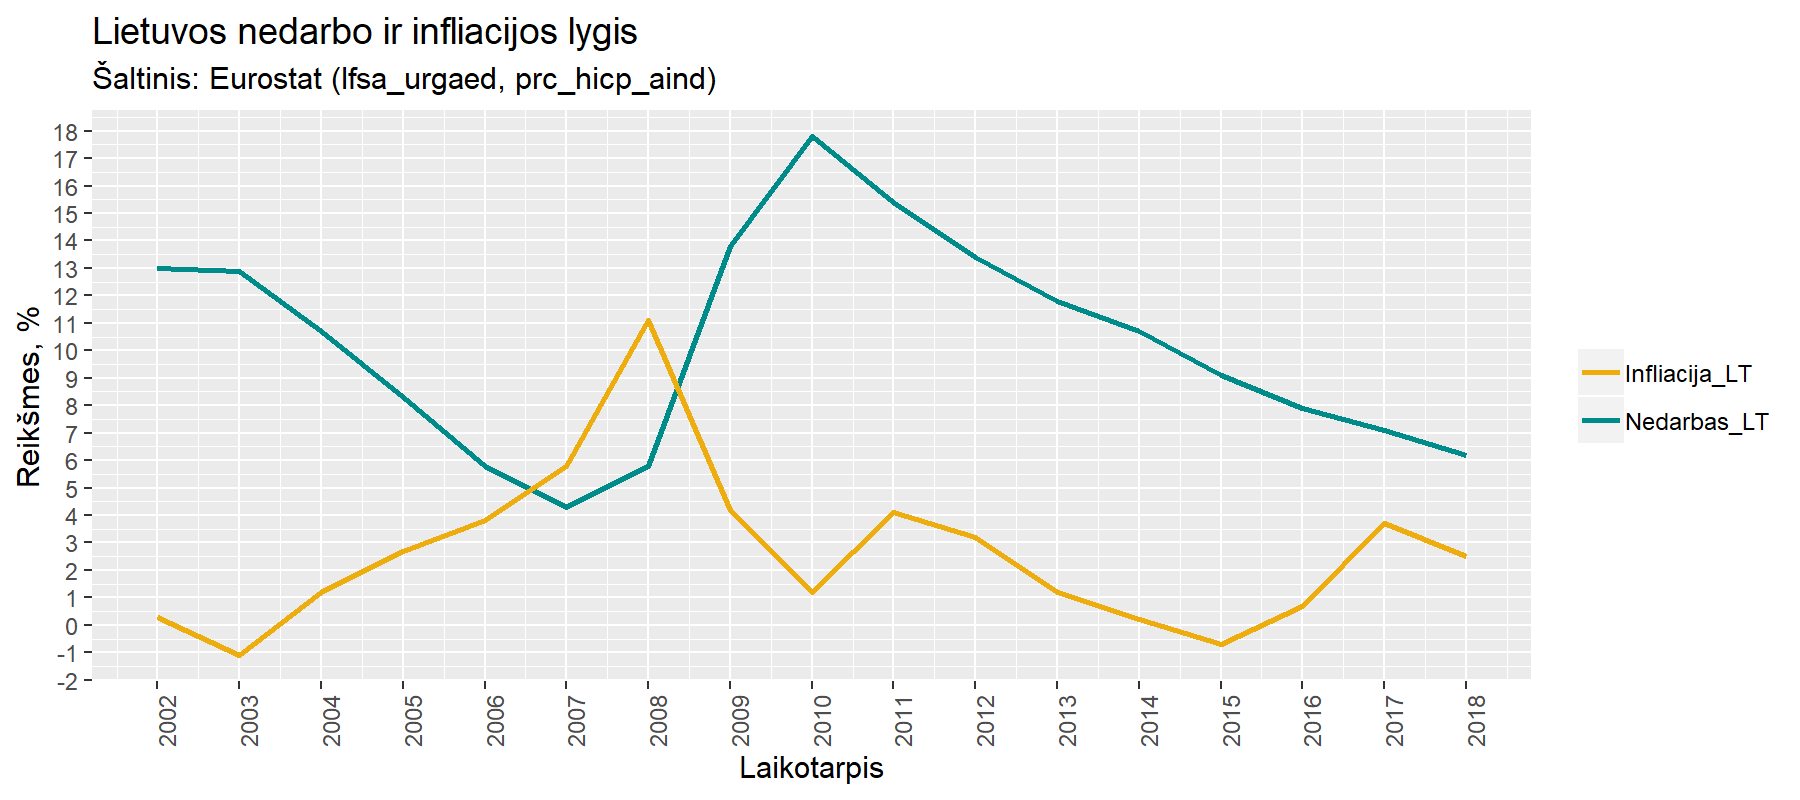
\includegraphics[scale=0.6]{Lietuvos_nedarbo_ir_infliacijos_lygis.png}

Taigi pradėkime nuo pirmojo grafiko „Lietuvos nedarbo ir infliacijos lygis“, kuris rodo ryšį tarp infliacijos dydžio ir nedarbo lygio Lietuvoje. Remiantis Phillips‘o teorija  infliacijos didėjimo metu turėtų mažėti nedarbo lygis, o infliacijos mažėjimo metu – nedarbo lygis turėtų didėti. Šis gautas grafikas rodo, jog nuo 2002 metų iki 2003 metų infliacija mažėjo smarkiai, tačiau kartu šiek tiek sumažėjo ir nedarbas. 2003-2007 metais pastebimas Phillips‘o teorijos pasitvirtinimas ir matomas infliacijos didėjimas ir kartu nedarbo mažėjimas. 2008 metais vėl galima matyti neatitikimą, didėja kartu ir infliacija ir nedarbo lygis. Remiantis istorijos žiniomis galima daryti prielaidą, jog taip įvyko dėl 2008 metais vykusios ekonominės krizės, kuri palietė Lietuvą. Vėliau 2009-2010 metais Phillips‘o teorija pradeda vėl galioti. Tačiau vėliau tik 2015-2017 metais atsiranda minėtasis ryšys tarp infliacijos ir nedarbo. Vertėtų paminėti, jog atvirkštinis ryšys tarp infliacijos ir nedarbo 2015 metais atsiranda po euro įvedimo Lietuvoje. Tačiau kitais laikotarpis atvirkštinio ryšio nėra.

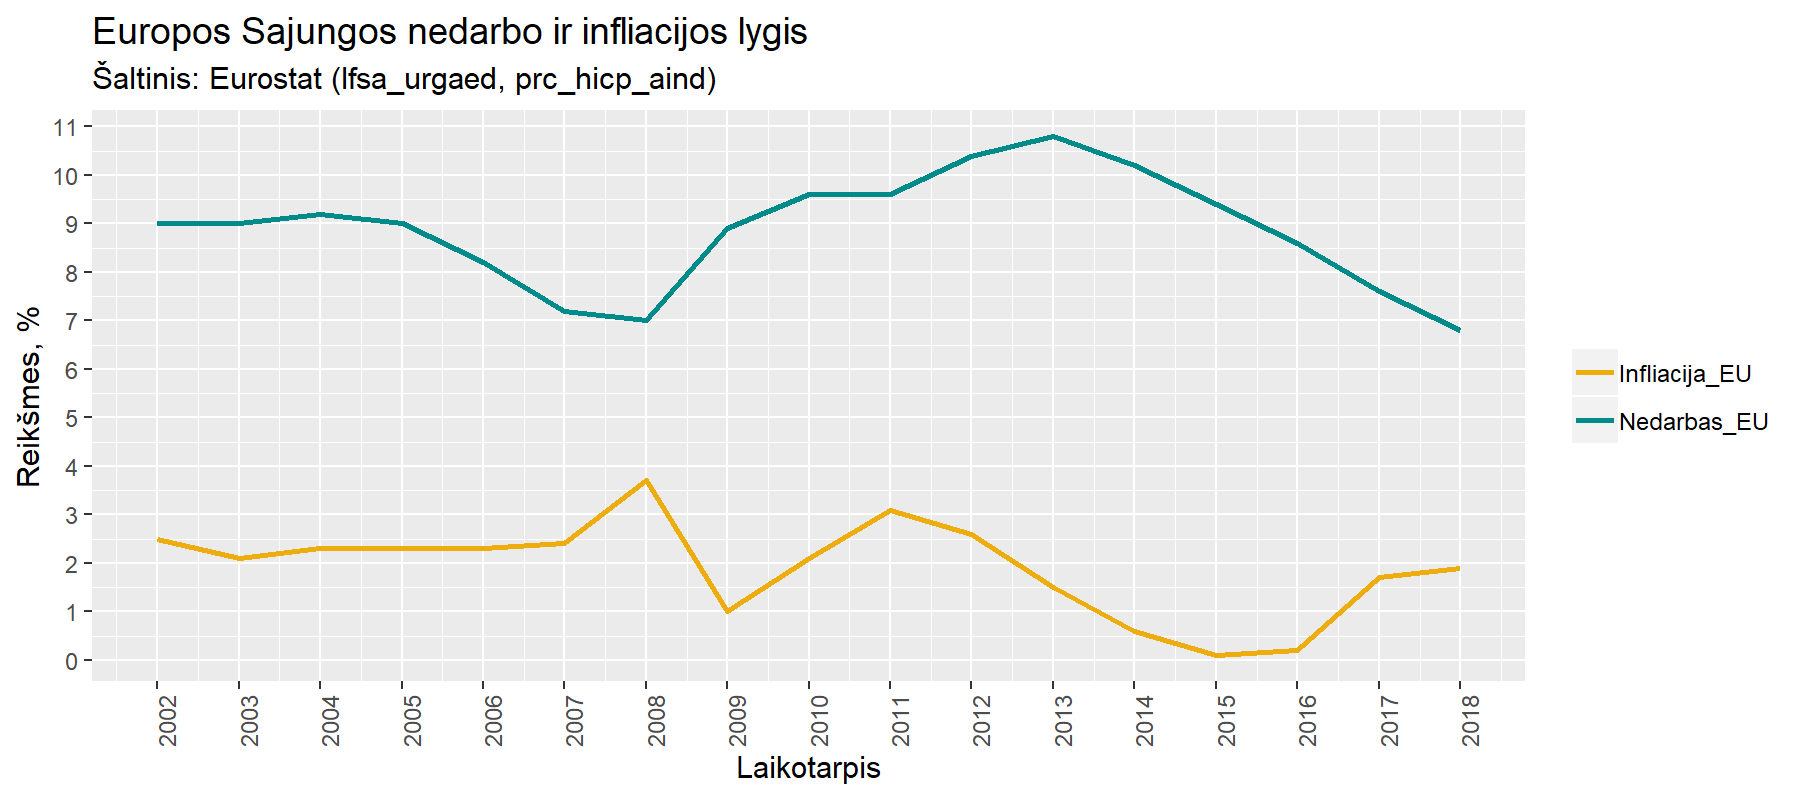
\includegraphics[scale=0.6]{EU_nedarbo_ir_infliacijos_lygis.png}

Pereinant prie „Europos Sąjungos nedarbo ir infliacijos lygio“ grafiko matyti panašios tendencijos kaip ir Lietuvoje. Reikėtų pastebėti, jog 2004-2007 metais infliacijos lygis Europos Sąjungoje yra ganėtinai pastovus, tačiau nedarbo lygis sparčiai mažėja. Be to, matyti, jog nuo 2017 metų atvirkštinis nedarbo ir infliacijos ryšys vėl tampa teisingas. Taip pat Europos sąjungoje beveik visu tiriamuoju laikotarpiu nedarbo lygis ganėtinai aukštas, o infliacijos žemas. Tačiau palyginus su Lietuvos duomenimis bendrai paėmus Europos Sąjungoje nedarbas daug mažesnis nei Lietuvoje. Taip pat lyginant Lietuvą ir Europos Sąjungą matyti, jog nuo 2017 metų ES yra atsirandantis atvirkštinis ryšys, tačiau Lietuvoje šio ryšio nėra.

Norėčiau pabrėžti, jog šios Phillips'o kreivės braižytos nurodant santykį tarp infliacijos ir nedarbo naudojantis R programa. Jeigu duomenis skaičiuotume pagal formules, nenaudojant R, duomenys galėtų šiek tiek skirtis.


\begin{figure}[h]
	\begin{minipage}[t]{3cm}
		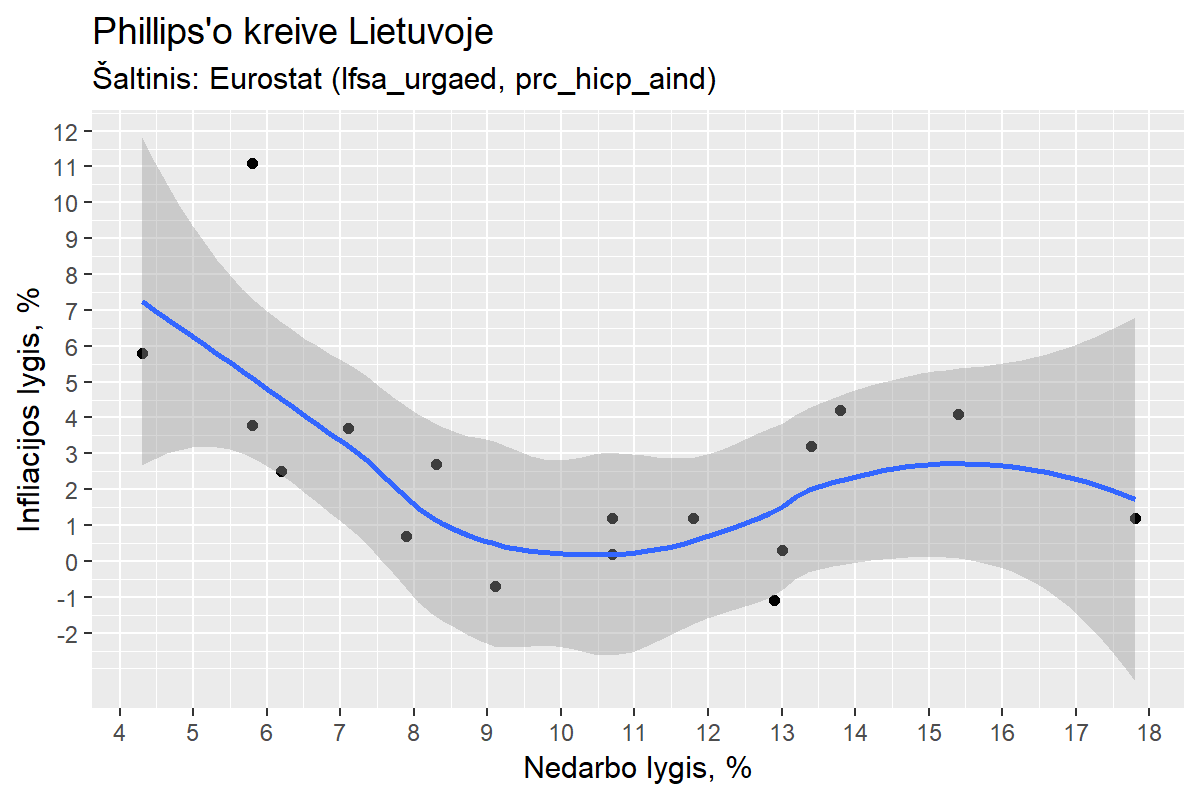
\includegraphics[scale=0.5]{LT_phillips.png}
	\end{minipage}
	\hspace{4cm}
	\begin{minipage}[t]{3cm}
		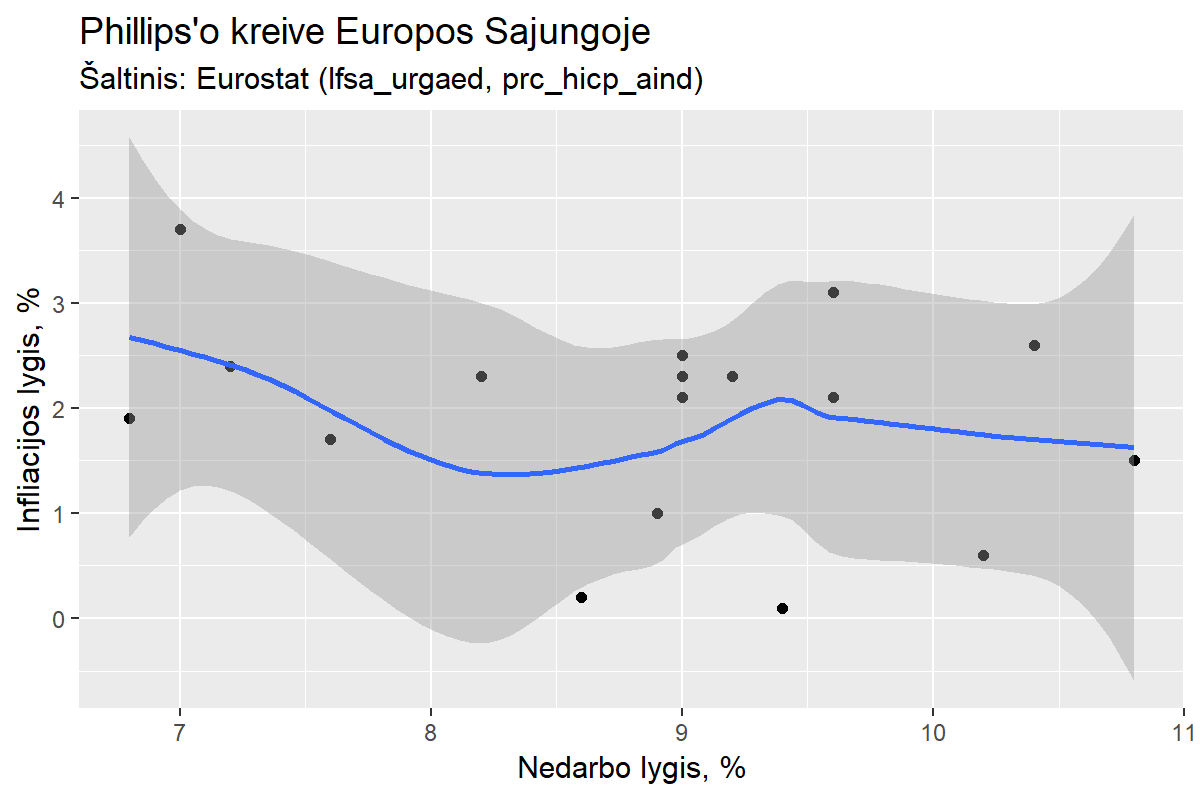
\includegraphics[scale=0.5]{EU_phillips.png}
	\end{minipage}
\end{figure}



Pagal gautą Lietuvos Phillips‘o kreivę galima matyti, jog atvirkštinis ryšys tarp infliacijos ir nedarbo lygio nėra pastovus. Iš pradžių matome, jog atitinka teoriją, tačiau vėliau atvirkštinis ryšys išnyksta. Remiantis ankstesniu infliacijos ir nedarbo Lietuvoje grafiku galima daryti prielaidą, jog neatitikimai gali būti maždaug nuo 2011 metų, kai infliacijos ir nedarbo lygiai mažėja kartu. Tuo tarpu vertinant gautą Europos sąjungos Phillips‘o kreivę galime taip pat matyti, jog Phillips‘o kreivė nėra pastovi ir atvirkštinys ryšys nevisada egzistuoja. Lygiai taip pat kaip ir Lietuvoje galima pastebėti, jog atvirkštinis ryšys dingsta ir kreivė tampa teigiama, nors vėliau atvirkštinis ryšys tarp infliacijos ir nedarbo lygio vėl atsiranda. 

\newpage
\section{Išvados}
Apibendrinant gautus grafikus ir išnagrinėtą teoriją, galiu pasakyti, jog sunku nustatyti ar Phillips‘o kreivė vis dar egzistuoja. Remiantis grafikais ne visada teisinga idėja, jog kylant infliacijos lygiui, nedarbo lygis mažėja, ir atvirkščiai. Gali būti, jog veikiant politiniams veiksniams, atsiradus naujiems stimulams infliacijos ir nedarbo pokyčiui - situacija pasikeičia. Imant tam tikrus laikotarpius puikiai matyti, jog atvirkštinis ryšys tarp infliacijos ir nedarbo yra. Tačiau esant pokyčiams tai sunku įvertinti ir galbūt labiau reikėtų palaikyti Phelps‘o modelį, jog ši kreivė nėra pastovi ir gali keistis priklausomai nuo tam tikrų veiksnių. Pagal šiuos mano grafikus, sunku vienareikšmiškai teigti, bet atrodo, jog Phillips‘o kreivė nustoja egzistuoti. Tačiau vienareikšmiškai atsakyti negalima, nes pagal ES grafiką nuo 2017 metų ryšys vėl pastebimas. Tačiau ryšio neatitikimo problema gali būti susijusi su tuo, jog kaip ir teigė Phelps‘as - ši kreivė veikia tik trumpuoju laikotarpiu. Manau, atlikus papildomus tyrimus būtų galima nustatyti ar ši kreivė nepasislinko į šoną ir nustatyti ar ji ir toliau egzistuoja.

\newpage

\bibliographystyle{apalike}
\bibliography{bibliography.bib}

\end{document}
